\section{コレクションを更新する}

私たちのアプリケーションは、新しい情報を受け取り、既存の情報を更新し、不要になった情報を削除するなど、常に外部と通信しています。しかし、これはClojureのイミュータブルなコア・コレクションと相反するように思えます。

Clojureでは、変化は常に純粋な関数をイミュータブルな値に適用し、その結果新しいイミュータブルな値が得られるというモデルになっています。言語学的なごまかしを避けるため、この変更手段を説明するために、単純な更新という言葉を使うことにします。

コレクションをイミュータブルに定義することには、多くの利点がある。まず、同時実行スレッドでは、値への参照ではなく、値の受け渡しが可能になる。これにより、他のスレッドによってデータが予測不可能に変更されることがない。第二に、ドメインロジックを状態管理機能から分離し、並行処理に関する問題をドメインデータや関数からきれいに分離します。

シーケンシャルなデータで発生する特殊なケースとして、キューのようにデータを更新する必要があります(先入れ先出し処理とも呼ばれる)。

\subsection{先入先出の処理}

ランチカウンターで、店員から注文が来ることを想像してください。公平性を保つために、注文は受け取った順に処理されることが期待されている - 先入れ先出し (FIFO) 処理。

Clojureでランチ・カウンターをモデル化するには、保留中のランチ・オーダーを保持するためのコレクションが必要です。ランチ・オーダーは時間的に自然な順序を持つので、リストやベクターのような連続したコレクションが必要なことが分かっています。ベクターを試してみましょう。

\begin{lstlisting}[numbers=none]
(defn new-orders [] [])

(defn add-order [orders order]
  (conj orders order))

(defn cook-order [orders]
  (cook (first orders)) (rest orders))
\end{lstlisting}

\texttt{add-order}関数は、\texttt{orders}の末尾に新しい\texttt{order}を追加しているので、vectorとしては効率的です。しかし、\texttt{orders}ベクターに対して\texttt{rest}を呼び出すのは非効率的です。これは、最初の要素以外のすべてを含むシーケンス(ベクターではない)を作成し、それを返します。もしベクターコレクション型を維持したければ、新しいベクターを構築し、そこにシーケンス要素を追加し直す必要があります;このすべてが高価です。

また、\texttt{orders}をリストで実装することもできる。\texttt{cook-order} のコードはそのままです。しかし、リンクされたリスト上で \texttt{rest} を呼び出すと効率的なので、ベクターで起こったパフォーマンスの問題に対処しています。しかし、\texttt{add-order}では新たな問題が発生しました。

\begin{lstlisting}[numbers=none]
(defn new-orders [] '())

(defn add-order [orders order]
  (concat orders (list order)))
\end{lstlisting}

リストの末尾にオブジェクトを追加する場合、リスト全体を走査して最後の要素を見つけ、新しいポインタを追加する必要があります。リストは先頭でのみ、ベクターは末尾でのみ効率的に追加と削除を行います。しかし、最後に追加し、最初に削除するコレクションが必要である。このニーズに応えるのが、次の図に示すようなキュー(待ち行列)です。

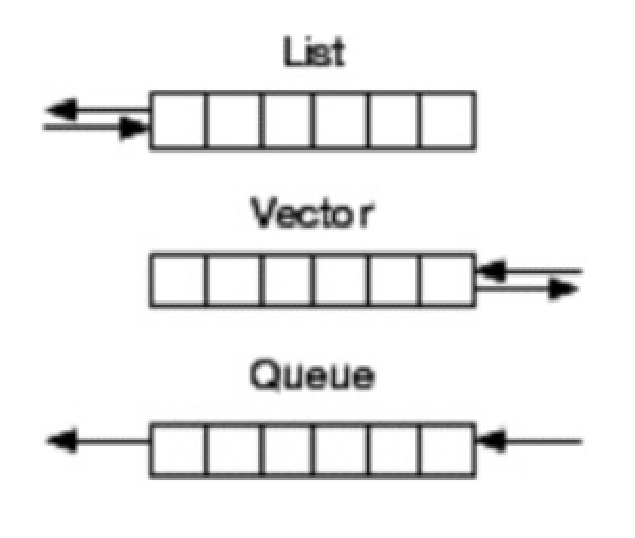
\includegraphics[width=5cm]{fig_02_001.eps}


他のすべてのコアコレクションと同様に、キューは不変の永続的なコレクションであり、リストやベクトルを扱うのと同じ関数をすべてサポートしています。以下は、ランチカウンターをキューで実装する方法です。

\begin{lstlisting}[numbers=none]
(def new-orders clojure.lang.PersistentQueue/EMPTY)

(defn add-order [orders order]
  (conj orders order))

(defn cook-order [orders]
  (cook (peek orders))
  (pop orders))
\end{lstlisting}

Clojureはリテラルなキューの構文やコンストラクタを提供しません。新しいキューを作成するには、静的な空のインスタンス \texttt{clojure.lang.PersistentQueue/EMPTY} で開始します。\texttt{add-order}では、vectorのように最後に新しい要素を追加するために\texttt{conj}を使用するだけです。\texttt{cook-order}では、最初の順序を見るために\texttt{peek}を使い、最初の順序以外を返すために\texttt{pop}を使います。

待ち行列の実装は、順序の追加と、待ち行列に入れられた順序での順序の削除の両方において効率的です。これは、この仕事に適したツールです。

次に、コレクションにデータを追加する処理を最適化する方法を考えてみましょう。


\subsection{一括インポート}

Clojureの永続的なコレクションは、イミュータブルです。効率化のために、\texttt{conj}や\texttt{assoc}のような関数で要素を追加すると、新しい不変の構造が作成されますが、その前と後のバージョンは通常そのデータの多くを共有します。コレクションは不変なので、これは安全に実行でき、データをコピーするよりもはるかに高速です。しかし、Clojureは制御されたコンテキストでミュータビリティを活用することで、より効率的にコレクションを埋める方法があります。

典型的なケースは、カタログアイテムのインポートです。アプリケーションが記録システムに直接アクセスできない場合、そのシステムからのエクスポートは、開始時にアプリケーションにインポートすることができます。カタログが変更されると、定期的な更新が必要になることは容易に想像できる。大規模なカタログの場合、その処理には時間がかかることがあります。

アプリケーションの起動時に呼び出される典型的なインポートを考えてみましょう。


\begin{lstlisting}[numbers=none]
(defn import-catalog [data]
  (reduce #(conj %1 %2) [] data))
\end{lstlisting}

変更できるようにして、誰にも知られずに多くの修正を加えることができたらどうでしょうか。Clojureのトランジェントがこれを可能にしてくれます。限られたスコープ内で、Clojureのコレクションを変更させることができます。

transientを呼び出すと、mutableバージョンのvector、hash-map、hash-setが得られます(オリジナルはimmutableのままです)。トランジェントコレクションはconjやassocのような永続的な変更関数では変更できません。 トランジェントコレクションにはインスタンスを変更する同等の関数セットがあり、すべて「\texttt{!}」接尾辞がつきます: \texttt{conj!}、 \texttt{assoc!}、などなどです。 読み込みインターフェイス(\texttt{get}、\texttt{contains?}など)は変更されずに動作し続けます。変更が完了したら、\texttt{persistent!}を呼んで、永続的なコレクションに戻ります。

以下は、transientコレクションを代わりに使用する\texttt{import-catalog}の更新版です。

\begin{lstlisting}[numbers=none]
(defn import-catalog-fast [data]
  (persistent!
    (reduce #(conj! %1 %2) (transient []) data)))
\end{lstlisting}

また、\texttt{item-data}にベクターのベクターとして読み込まれた約100万点のカタログアイテムをインポートしているときの速度を、時間を使って2つのバージョンの性能差を確認することができます。

\begin{lstlisting}[numbers=none]
catalog-import.core=> (time (import-catalog item-data)))
"Elapsed time: 129.602 msecs"
catalog-import.core=> (time (import-catalog-fast item-data)))
"Elapsed time: 110.104 msecs"
\end{lstlisting}

トランジェントは、バルクインポートを行う際に大きな力を発揮します。Clojureのinto関数が変換コレクションを取り、それがトランジェントにできるかどうかを判断するのはこのためです。もしそうなら、出力コレクションは自動的にトランジエントにされ、トランジエント関数を使用して充填され、永続的なコレクションに戻されます。

リストとベクター内の要素は、通常、更新されない。その代わり、シーケンシャルなコレクションでは、コレクションの挿入ポイントで要素の追加と削除を行うことがほとんどです。しかし、マップの内部内容は頻繁に更新され、マップはいくつかの一般的な方法で変換される必要がある。

\subsection{マップの更新}

マップを修正する基本的なツールは\texttt{assoc}と\texttt{dissoc}です。 \texttt{assoc}関数はキーに新しい値が供給されると、その値を更新します。Clojure 1.7では、関数の適用に基づいてキーの値を変換することができる\texttt{update}関数が追加されました。

例えば、宇宙シミュレーションの惑星の1つを記述するエンティティ(適切なマップ・インターフェイスも実装しています)を考えてみましょう。



\begin{lstlisting}[numbers=none]
(def earth {:name       "Earth"
            :moons      1
            :volume     1.08321e12 ;; km^3
            :mass       5.97219e24 ;; kg
            :aphelion   152098232  ;; km, farthest from sun
            :perihelion 147098290  ;; km, closest to sun
           }
\end{lstlisting}

ユーザーがシミュレーションに月を追加した場合の効果を調べるための機能を追加することを検討します。\texttt{update}関数を使って、月の数を増やす\texttt{inc}関数を適用することができます。


\begin{lstlisting}[numbers=none]
(update earth :moons inc)
\end{lstlisting}

\texttt{update}関数は、コレクション内の値に関数を適用し、その結果として更新されたコレクションを受け取るという処理をカプセル化したものです。

時には、マップ内の1つの値だけでなく、多くの値を同時に更新する必要があります。多くの場合、実体を表すマップは、CSVファイル、JSONデータ、データベースなどの外部データソースから取り込まれます。キーはキーワードではなく文字列であったり、キーワードが間違った名前空間や大文字小文字であったりと、求めるものと異なる形式であることがある。

Clojureコア・ライブラリには、マップ内のすべてのキーを更新するための単一の関数はまだ含まれていませんが、多くの外部ユーティリティ・ライブラリが解決策を提供しています。ここでは、多くの開発者が便利だと思う少数の関数を含む \texttt{Medley} ライブラリを使用します。

例えば、以下のような形式の文字列キーを持つJSONソースから惑星データを受信することを考える。


\begin{lstlisting}[numbers=none]
{"name" "Earth"
 "moons" 1
 "volume" 1.08321e12
 "mass" 5.97219e24
 "aphelion" 152098232
 "perihelion" 147098290}
\end{lstlisting}

\texttt{Medley}の\texttt{map-keys}関数を使って、このエンティティのキーを全て変更することができます。

\begin{lstlisting}[numbers=none]
(:require [medley.core :refer (map-keys)])
\end{lstlisting}

\begin{lstlisting}[numbers=none]
(defn keywordize-entity [entity]
  (map-keys keyword entity))

(keywordize-entity {"name"   "Earth"
                    "moon"   1
                    "volume" 1.08321e12
                    "mass"   5.97219e24
                    "aphelion" 152098232
                    "perihelion" 147098290})
;; {:name "Earth",
;;  :moons 1,
;;  :volume 1.08321E12,
;;  :mass 5.97219E24,
;;  :aphelion 152098232,
;;  :perihelion 147098290}
\end{lstlisting}

おそらくもっと一般的なのは、マップをインデックスとして使用する場合、1回の呼び出しですべてのマップの値を更新する必要があることでしょう。\texttt{Medley}ライブラリには、この目的のために\texttt{map-vals}関数も用意されています。

モデリングの関係で考えたレシピのインデックスがレシピ識別子からレシピへのマップであったことを思い出してください。もし私たちがインデックス内のすべてのレシピにカロリー情報を追加する必要があるならば、次のように\texttt{map-valsas}を使うことでレシピのインデックスを更新することができます。レシピの総カロリー数を生成できる\texttt{compute-calories}関数を持っていると仮定します。

\begin{lstlisting}[numbers=none]
(:require [medley.core :refer (map-vals)])
\end{lstlisting}


\begin{lstlisting}[numbers=none]
(defn- update-calories
  [recipe]
  (assoc recipe :calories (compute-calories recipe)))

(defn include-calories
  [recipe-index]
  (map-vals update-calories recipe-index))
\end{lstlisting}

まず、\texttt{update-calories}ヘルパー関数を定義します。これは、新しい\texttt{:calories}フィールドを計算し、単一のレシピに関連付けるために使用されます。それから、\texttt{include-calories}で、マップのすべての値にこの関数を適用するために\texttt{map-vals}を使用します。
   
マップのすべてのキーや値を更新するこれらの単純な関数は驚くほど便利で、ほとんどのプロジェクトは最終的にこれらのユーティリティを書いたり、含めたりしています。\texttt{Medley}では、これらの関数の実装にトランジェントを使用してパフォーマンスを向上させています。トランジェントの利点は、Bulk Importでご覧いただいたとおりです。

\texttt{Medley}には他にも、\texttt{filter-keys}、\texttt{filter-val}、\texttt{remove-keys}、\texttt{remove-val}という便利なマップ変換関数がいくつかあります。これらは、述語関数(ブール値を返す)を適用した結果に基づいて、マップエントリのサブセットを保持または削除することができます。

さて、コレクションを選んでデータを入れたら、次はそこからデータを取り出す方法を考えましょう。

